\chapter{Architecture\label{sec:architecture}}
Après avoir fait un tour d'horizon des différents modules, je vous propose
d'étudier l'architecture complète du programme.

\remark{Bien qu'il ne s'agisse pas vraiment de modules (ce concept n'existe pas
en C++), il existe tout de même des groupements de classes qu'il soit
sémantique ou fonctionnel. C'est ce que j'assimilerai comme définition pour
``module''.}

\section{Camera}
L'ensemble des caméras doivent respecter l'interface de la \tsl{fig.
\ref{fig:ICamera}}. Concrètement, chaque caméra doit pouvoir, à partir des
coordonnées de l'espace écran (coordonnées UV), fournir l'ensemble des rayons
nécessaires au dessin de la scène.

\begin{figure}[h]
  \inputcode{c++}{../../code/src/Cameras/Camera.hpp}
  \caption{Code de l'interface commune à toutes les
  caméras\label{fig:ICamera}}
\end{figure}

\subsection{Spécialisations}
\paragraph{[Implémentée] Caméra perspective} Une caméra simple avec gestion de
la perspective.

\paragraph{[Implémentée] Caméra perspective DOF} Une caméra avec
gestion de la perspective et rendu de l'effet de profondeur de champs (\cf
\tsl{section \ref{sec:dof}}).

\paragraph{[Non implémentée] Caméra orthographique} Caméra avec projection
orthographique (utiles pour les rendu de pièce en 3D et le métrage).

\paragraph{[Non implémentée] Caméra fish eye} Cette caméra permet d'utiliser
des matrices de projection grand angle.

\begin{figure}[h]
\begin{center}
  \noindent\makebox[\textwidth]{%
    \includegraphics[width=1.5\textwidth]{../../architecture/Cameras}}
  \caption{Diagramme de classe du module Caméra\label{fig:CDCamera}}
\end{center}
\end{figure}
 % CHECKED
\clearpage

\section{Sampler}
Les \tsl{samplers}\ ont pour objectif d'échantillonner le nombre de rayons
lancés pour chaque pixel. Pour cela, il est nécessaire de leur fournir toute
la scène car ils nécessitent au moins la caméra mais peuvent avoir besoin de
beaucoup d'autre éléments (par exemple, l'ensemble des géométries). Il est par
exemple possible de \tsl{supersampler}, \ie lancer plus de rayons qu'il ne
semble nécessaire afin d'éviter les phénomènes de crénelage.\\

Encore une fois, les \tsl{samplers}\ doivent respecter la même interface
définit à la \tsl{fig. \ref{fig:ISampler}}.

\begin{figure}[h]
  \inputcode{c++}{../../code/src/Samplers/Sampler.hpp}
  \caption{Code de l'interface commune à tous les
  samplers\label{fig:ISamplers}}
\end{figure}

\subsection{Spécialisations}
\paragraph{[Implémentée] DefaultSampler} Ce \tsl{sampler}\ lance un seul rayon
par pixel.

\paragraph{[Implémentée] SuperSampler} Ce \tsl{sampler}\ lance $N$ rayons par
pixel où $N$ est passé en paramètre.

\paragraph{[Non implémentée] Adaptative sampling} Il existe un \tsl{sampler}\
que je n'ai pas eu le temps d'implémenter et qui pourtant définit la stratégie
la plus intelligente d'échantillonnage. Il s'agit de l'échantillonnage
adaptatif qui, tant que la moyenne des pixels environnant est supérieure à un
certain seuil de différence, lance des rayons selon une distribution
statistique.

\vspace*{\fill}
\begin{figure}[h]
\begin{center}
  \noindent\hbox to \textwidth
  {\hss\includegraphics[width=1.5\textwidth]{../../architecture/Samplers}\hss}
  \caption{Diagramme de classe du module Sampler\label{fig:CDSamplers}}
\end{center}
\end{figure}
 % CHECKED
\clearpage

\section{Lumières}
L'ensemble des sources de lumières doivent respecter l'interface de la \tsl{fig.
\ref{fig:ILights}}. Concrètement, chaque caméra doit pouvoir, à partir des
coordonnées de l'espace écran (coordonnées UV), fournir l'ensemble des rayons
nécessaire au dessin de la scène.

\begin{figure}[h]
  \inputcode{c++}{../../code/src/Lights/Light.hpp}
  \caption{Code de l'interface commune à toutes les
  sources de lumières\label{fig:ILights}}
\end{figure}

\subsection{Spécialisations}
\paragraph{[Implémentée] Lumière directionnelle} Cette source éclaire tout selon une
direction passée en paramètre.

\paragraph{[Implémentée] Lumière ponctuelle} Cette source, définit grâce à sa position,
rayonne autour d'elle comme une sphère lumineuse.

\paragraph{[Implémentée] Lumière surfacique plane} Cette source a la particularité d'avoir une
composante surfacique ce qui permet de générer des ombres douces (\cf
\tsl{section \ref{sec:softshadows}}).

\paragraph{[Non implémentée] Cone de lumière}

\paragraph{[Non implémentée] Autre lumières surfaciques} Il est possible de
rajouter tout les types de lumières surfaciques comme des sphères lumineuse et
même des mesh lumineux. 

\subsection{Diagramme de classe}
\begin{figure}[h]
\begin{center}
  \includegraphics[width=\textwidth]{../../architecture/Lights}
  \caption{Diagramme de classe du module Light\label{fig:CDLights}}
\end{center}
\end{figure}
 % CHECKED
\clearpage

\section{Geometry}
Ce module regroupe l'ensemble des géométries que le programme peut calculer.
Chacune de ces classes doivent respecter l'interface définit à la
\tsl{fig. \ref{fig:IGeometry}}.

\begin{figure}[h]
  \inputcode{c++}{../../code/src/Geometry/Geometry.hpp}
  \caption{Code de l'interface commune à toutes les
  géométrie \label{fig:IGeometry}}
\end{figure}

\subsection{Spécialisations}
\paragraph{[Implémentée] Sphère}
\paragraph{[Implémentée] Plane}
\paragraph{[Implémentée] Box} Cette géométrie est uniquement utilisée pour la
structure d'Octree.

\paragraph{[Implémentée] Triangle}

\paragraph{[Implémentée] Mesh} Qui est en réalité un aggrégat de triangles
stockés dans un octree.

\paragraph{[Non implémentée] Quadric} Les \tsl{quadrics} sont un ensemble de
géométrie paramétré par une équation de la forme $$xQx^T + Px^T + R = 0$$. 

Cette équation permet de décrire tout une gamme de forme allant de l'ellipse à
la sphère en passant par plusieurs types de cônes.\footnote{Pour la liste
complète, je vous invite à consulter
\url{http://en.wikipedia.org/wiki/Quadric}.}.

\subsection{Diagramme de classe}
\begin{figure}[h]
\begin{center}
  \includegraphics[width=\textwidth]{../../architecture/Geometries}
  \caption{Diagramme de classe du module Geometry\label{fig:CDGeometry}}
\end{center}
\end{figure}
 % CHECKED
\clearpage

\section{Builder}
Chaque objet constructible doit aussi définir un \tsl{builder}, \ie une classe
permettant à partir de la description textuelle de l'objet (\cf section
\ref{sec:scenemanager}), de construire sa représentation mémoire.

L'interface à respecter est celle présentée à la \tsl{fig.
\ref{fig:IBuilders}}.

\begin{figure}[h]
  \inputcode{c++}{../../code/src/Builders/Builder.hpp}
  \caption{Code de l'interface commune à tous les
  \tsl{builders}\label{fig:IBuilders}}
\end{figure}


\subsection{Spécialisations}
Un pour chaque objet constructible. On peut citer \ttt{MaterialBuilder},
\ttt{SphereBuilder}, \ttt{DirectionalBuilder}, \etc

\begin{figure}[h]
\begin{center}
  \vspace*{-4cm}
  \includegraphics[angle=90,width=.4\textwidth]{../../architecture/Builders}
  \caption{Diagramme de classe du module Sampler\label{fig:CDBuilders}}
\end{center}
\end{figure}
 % CHECKED
\clearpage

\section{Scene}
Pour être construite, la scène doit lire un fichier au format XML (\cf
\tsl{section \ref{sec:scenemanager}}).\\

Une scène contient les champs suivant :
\begin{itemize}
  \item Une caméra
  \item Une liste de matériaux
  \item Une liste de géométries
  \item Une liste de lumière.
  \item Une couleur ambiante,\ie la ``couleur du vide''.
  \item L'image où sera écrite le rendu.
\end{itemize}

Lors de la création, le programme lit le fichier XML et appelle successivement
tous les \tsl{builders} disponible afin d'en trouver un capable de construire
la représentation mémoire de l'objet.
 % CHECKED
\clearpage

\section{Image}
La manipulation des images est évidemment au cœur du programme. Il doit être
capable de lire (pour les textures) et d'écrire (pour le rendu) plusieurs
formats d'image.

Pour cela, l'architecture du module est basé autours d'un \tsl{Builder} (\cf
\cite{DesignPatternsBook}, \tsl{p. 97}) dont une seule instance est autorisée
(\tsl{design pattern Singleton, p. 127}). Ainsi, il est possible de créer une
collection de classes capables de manipuler différents formats d'images. Par la
suite, le \tsl{Builder} pourra choisir la bonne implémentation des méthodes de
chargement et de sauvegarde de l'image correspondant au format demandé.

\subsection{Spécialisations}
\paragraph{[Implémentée] PNGHandler} Permet de manipuler le format PNG.

\paragraph{[Implémentée] JPGHandler} Permet de manipuler le format JPG. 

\paragraph{[Non implémentée] Autre} Il existe plusieurs dizaines de formats
qu'il faudrait supporter.

\begin{figure}[h]
\begin{center}
  \includegraphics[width=.4\textwidth]{../../architecture/ImageHandlers}
  \caption{Diagramme de classe du module Image\label{fig:CDImageHandlers}}
\end{center}
\end{figure}
 % CHECKED
\clearpage

\section{Architecture complète}
La figure \ref{fig:archiAll} présente l'architecture des principaux modules du
programme. Malheureusement, il est impossible de présenter sous forme
intelligible l'ensemble des interactions et pour cette raison, je vous invite
à consulter la documentation \tsl{Doxygen} qui parvient bien mieux que moi à
mettre en valeurs les relations entres les classes.

\begin{figure}[p]
  \vspace*{-4cm}
  \hbox to \textwidth
  {\hss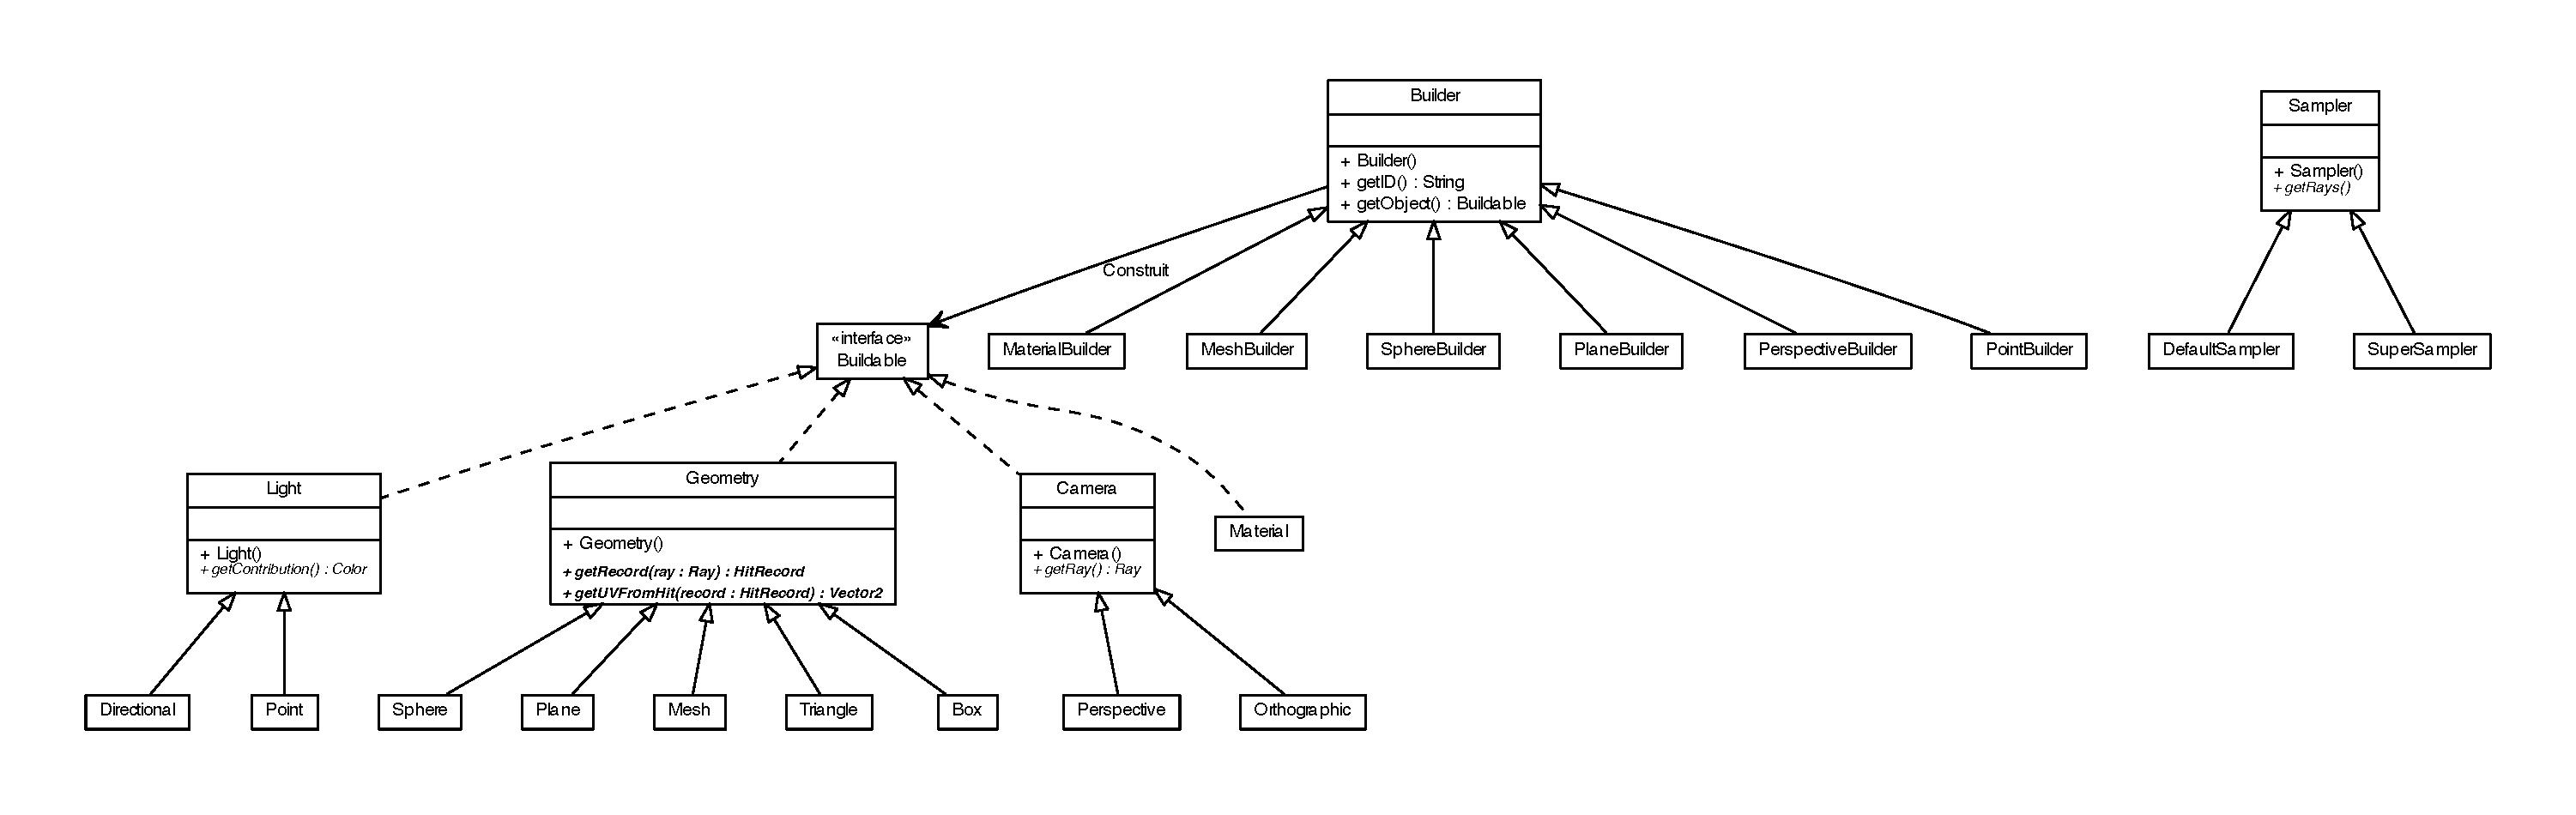
\includegraphics[angle=90,width=.6\textwidth]{../../architecture/LRT.pdf}\hss}
\end{figure}
